\documentclass[dwyatte_dissertation.tex]{subfiles} 
\begin{document}

\chapter{Neural model of spatiotemporal prediction for object recognition}

\section{Introduction}
TODO

\section{Methods}

\subsection{Model architecture}

The model consisted of three layers and one preprocessing stage whose parameters are described in detail in the following paragraphs. Two of the layers contained columnar substructure which was necessary for implementing learning using the LeabraTI framework (Chapter \ref{chap:leabrati}). To simplify the overall LeabraTI computation, only superficial (Layers 2 and 3) and deep (Layer 6) neuron subtypes were explicitly modeled. Projections between these neuron populations correspond to the descending Layer 5 $\rightarrow$ Layer 6 synapses in the brain, which are assumed to be plastic, and the ascending Layer 6 $\rightarrow$ Layer 4 transthalamic synapses which are assumed to be relatively stable and nonplastic.

% model fig
\begin{figure}[h!]
\begin{center}
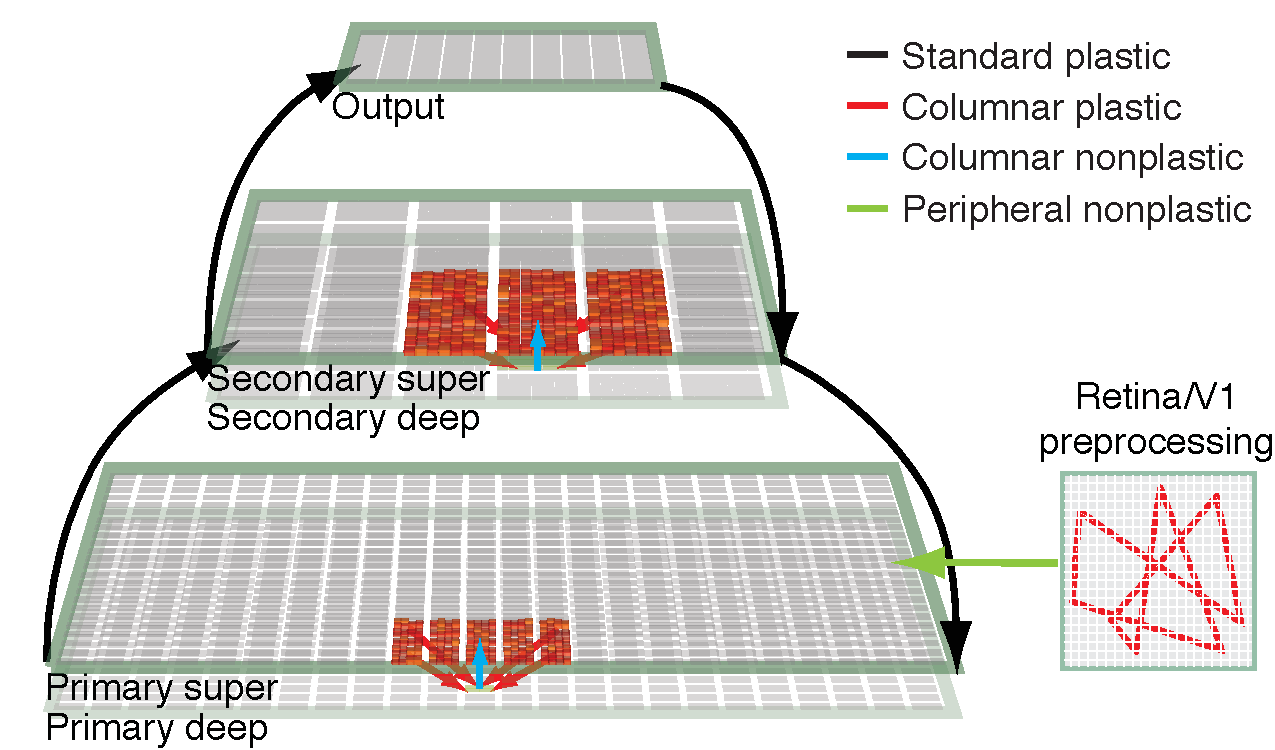
\includegraphics[width=160mm]{figs/chap_sims/v1_v2_output_ti_annotated.pdf}
\end{center}
\caption{Model architecture}{The model's four layers and principal projections. Primary and secondary visual layers contained columnar substructure in which deep units integrated from 5x5 columns of superficial units in the primary case or 3x3 columns in the secondary case. Ascending synapses from deep to superficial units were nonplastic and connected in a one-to-one manner.}
\label{fig:v1_v2_output}
\end{figure}

\textbf{Retina and V1 preprocessing:} Input was provided to the model via a 24x24 topographic filter bank that preprocessed images offline from the model proper. This preprocessing step is consistent with a large class of biological models describing object recognition in cortex \cite[e.g.,]{RiesenhuberPoggio99,SerreOlivaPoggio07,OReillyWyatteHerdEtAl13} and in the case of the present model, represents visual processing from the level of the retina through V1 simple cells \cite{HubelWiesel62}. Grayscale bitmap images were scaled to 24x24 pixels and convolved with Gabor filters at four orientations (0$^\circ$, 45$^\circ$, 90$^\circ$, and 135$^\circ$) and two polarities (off-on and on-off) producing a 24x24x4x2 set of inputs. Each Gabor filter was implemented as 6x6 pixel kernel, with a wavelength $\lambda$ = 6 and Gaussian width terms of $\sigma_x$ = 1.8 and $\sigma_y$ = 1.2. A static nonlinearity was applied to the output of the filtering step in the form of a modified \textit{k}-Winners-Take-All (\textit{k}WTA) inhibitory competition function that reduced activation across the 4x2 filter bank to the equivalent of \textit{k} = 1 fully active units \cite[see][Supporting Information]{OReillyWyatteHerdEtAl13}.

\textbf{Primary visual layers:} 24x24 topographic layer arranged into groups of 4x2 units (4608 total units), decomposed into superficial and deep neuron subtypes. Each superficial unit received the output of the retina/V1 preprocessing step. \textit{k}WTA inhibition for superficial units was set to 60\% of the average of the top \textit{k} active units compared to the average of all other superficial units with each 4x2 unit group using a value of \textit{k} = 2. Deep units received from 5x5 columns of superficial units (200 inputs per deep unit) integrated into a single value that was used as the additional context input channel for each superficial unit.

\textbf{Secondary visual layers:} 6x6 topographic layer arranged into groups of 7x7 units (1764 total units), also decomposed into superficial and deep neuron subtypes. Each superficial unit received from 8x8 topographical neighborhoods of early visual columns (512 afferents per unit) and sent back reciprocal connections with the same topography. \textit{k}WTA for superficial units was set to 60\% of the average of the top \textit{k} active units compared to the average of all other superficial units with each and 15\% activity within each unit group. Deep units received from 3x3 columns of superficial units (441 inputs per deep unit) integrated into a single value that was used as the additional context input channel for each superficial unit.

\textbf{Output layer:} 10x10 layer (100 total units) without unit group or columnar substructure. Each unit received a full projection from secondary visual columns (1764 afferents per unit) and fully projected back to all columns. A scalar of 10\% was used to limit the influence of the output units on secondary visual columns during the training period, preventing runaway representation that can become disconnected from bottom-up inputs. A \textit{k}WTA value of \textit{k} = 1 was used to enforce a localist representation. The localist representation is a computational simplification that allowed an identity readout of lower-level features without population decoding similar to that provided by inferior temporal (IT) neurons  \cite{HungKreimanPoggioEtAl05,LiCoxZoccolanEtAl09}. 

\subsection{LeabraTI learning algorithm}

LeabraTI was implemented as an extension of the standard Leabra algorithm which is described in detail in \incite{OReillyMunakata00} and \incite{OReillyMunakataFrankEtAl12}. Standard Leabra learning operates across two phases: a \textit{minus} phase that represents the system's expectation for a given input and a \textit{plus} phase, representing observation of the outcome. The difference between the minus and plus phases, along with additional self-organizing mechanisms, is used in computing the synaptic weight update function at the end of each plus phase. 

LeabraTI extends standard Leabra learning by interleaving its minus and plus phases over temporally contiguous input sequences. In standard Leabra, the minus phase depends on clamped inputs from the sensory periphery to drive the expectation while the plus phase uses clamped outputs from other neural systems to drive the outcome. In LeabraTI, the minus phase expectation is not driven by the sensory periphery, but instead by lagged context represented by deep (Layer 6) neurons. During the plus phase, driving potential shifts back to the sensory periphery. Deep neurons' context is also updated after each plus phase.

LeabraTI was only used to update the synaptic weights between superficial and deep neurons. Inter-areal feedforward and feedback projections bifurcate from the local column, directly synapsing disparate populations of superficial neurons and thus weight updates in these cases were handled by standard Leabra equations. In computing the weight update, the standard Leabra delta rule \cite{OReilly96} uses the difference in rate between the plus and minus phases of receiving units (\textit{y}) in proportion to the rate of sending units (\textit{x}) in the minus phase:
\begin{align*}
\Delta_{leabra} w_{ij} &= x^-(y^+ - y^-)
\end{align*}

In the LeabraTI framework, deep neurons are considered to be the receiving units as they are the terminus of the descending columnar synapses. However, deep units are proposed to only be active during the minus phase when they drive the prediction, and thus cannot be used to compute an error signal.  To address this issue, we invert the LeabraTI delta rule:
\begin{align*}
\Delta_{leabrati} w_{ij} &= super^-(deep^+ - deep^-) \\
			  &\approx deep^-(super^+ - super^-)
\end{align*}

Additionally, the temporally extended nature of the algorithm requires that the receiving units represent the current state (time \textit{t}) and sending units the previous moment's state (time \textit{t} - 1). While conceptualized as the previous equation, the actual implementation is as follows:
\begin{align*}
\Delta_{leabrati} w_{ij} &= super_{t-1}^+(super_{t}^+ - super_{t}^-)
\end{align*}

This formulation allows the driving potential of deep neurons to be computed just once using the previous plus phase state of superficial neurons (multiplied by the superficial $\rightarrow$ deep learned weights) and held constant as an input to superficial neurons during the minus phase. This is a gross simplification of the actual biological process of deep neurons, but is vastly more computationally efficient than explicit modeling by computing an additional rate for each deep neuron at each time step. This formulation is also equivalent to the simple recurrent network (SRN) \cite{Elman90,Servan-SchreiberCleeremansMcClelland91}, thus providing a potential biological substrate for its computational function. 

One limitation of LeabraTI's interleaving of minus and plus phases over time is that the initial minus phase in an input sequence does not have access to the previous moment's  context. Even if there was lagged context available, it would represent information from a prior, possibly unrelated input sequence. To address this, weight updates are disabled for the first minus-plus phase pair, and enabled thereafter. In the brain, this process might be facilitated by a neural mechanism that is sensitive to the repetition of inputs over time (e.g., acetylcholine) \cite{ThielHensonMorrisEtAl01,ThielHensonDolan02}.

\subsection{Training and testing environment}
% 50 cycles -, 20 +
The same four ``paper clip'' objects used in the Chapter \ref{chap:bpleast} experiment were used in training and testing the model. During training, an input sequence depicted one of the four objects rotating coherently through all 30 view renderings (adjacent views spaced 12$^\circ$ apart). During the minus phase, the model made a prediction about the upcoming view and during the plus phase, the view was processed by the retina/V1 filter banks and clamped as an input to the model. The output unit corresponding to each object was also clamped during the plus phase to bias views belonging to the same object toward similar lower-level feature representations. Training proceeded for 20 epochs of 10 randomly selected input sequences each. The learning rate on all plastic projections started at 1.0 and was halved every 8 epochs.

Training efficacy was evaluated by computing the average cosine (normalized dot product) between the minus and plus phase for the primary and secondary visual layers:
\begin{align*}
cos \theta = \frac{1}{n}\sum_{k=1}^{n}\frac{layer_k^- \cdot{} layer_k^+}{||layer_k^-||||layer_k^+||}
\end{align*}

The cosine varies between 0 and 1 and expresses the degree of similarity of LeabraTI's prediction to the actual outcome in layers with columnar substructure (Figure \ref{fig:v1_v2_output_train}). A value of zero indicates the minus phase prediction is completely orthogonal to the plus phase sensation and a value of 1 indicates complete overlap. The lower-bound on the cosine is not likely to be zero as it would require spurious activations in topographic regions that do not contain any features. A better approximation of the lower bound is the case when the system simply reproduces the plus phase from the previous moment's (\textit{t} - 1) state. This can be thought of as the amount of perceptual overlap between adjacent views of the stimuli, and thus any additional features that contribute to a higher cosine value indicate positive prediction.

% training fig
\begin{figure}[h!]
\begin{center}
\begin{tabular}{ll}
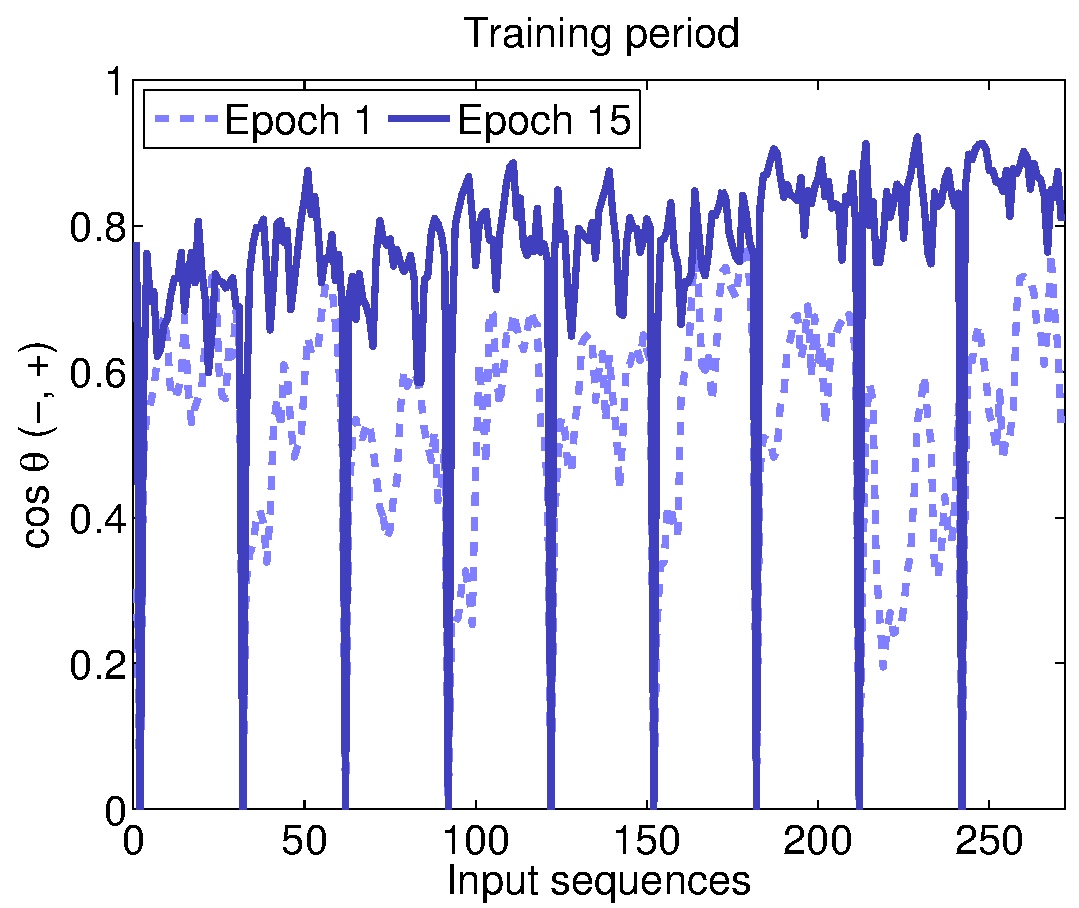
\includegraphics[width=80mm]{figs/chap_sims/sims_cos_out_trl.pdf}
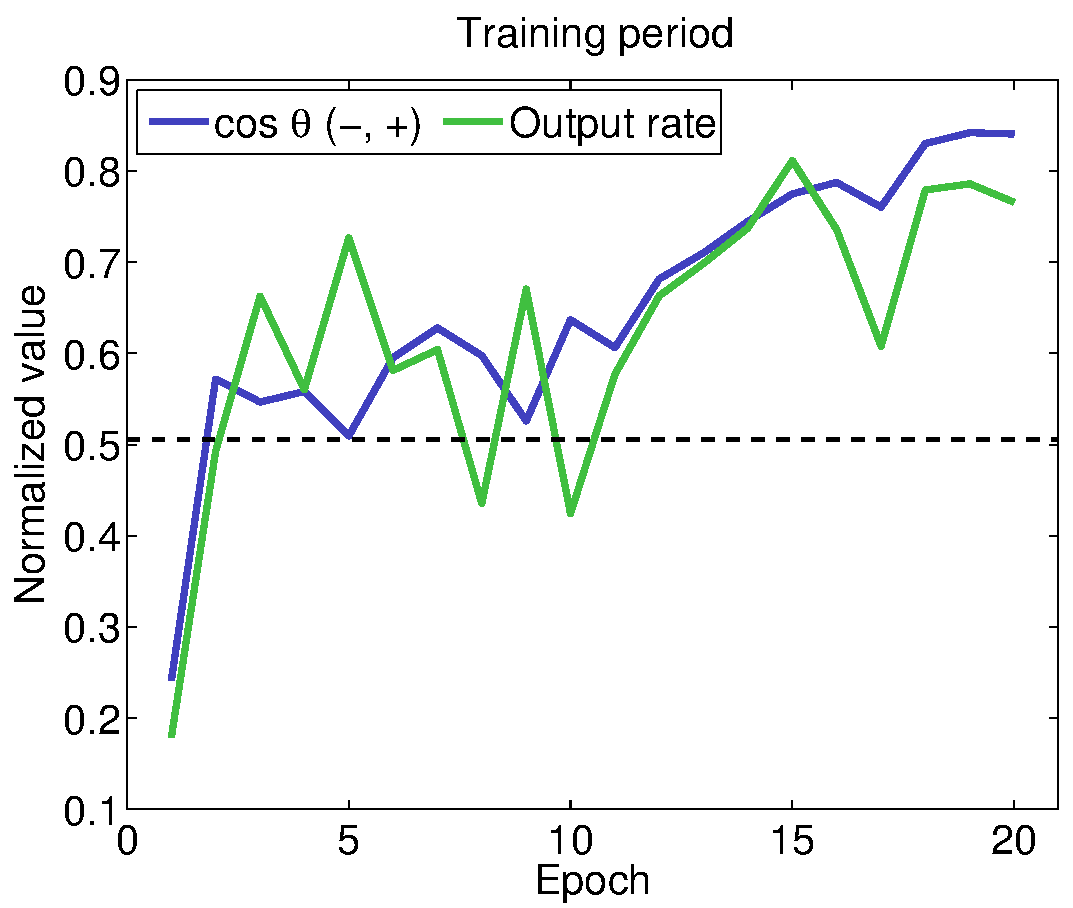
\includegraphics[width=80mm]{figs/chap_sims/sims_cos_out_epc.pdf}
\end{tabular}
\end{center}
\caption{Model training}{Average cosine between minus and plus phase for layers with columnar substructure and output response rate over the course of training. Sharp drops in the cosine to zero indicate the start of a new input sequence and are unlearnable. The lower bound for the cosine was computed as the reproduction of the plus phase from the previous moment's (\textit{t} - 1) state and the overall average is indicated by the dotted line. A cosine greater than this level indicates positive prediction.}
\label{fig:v1_v2_output_train}
\end{figure}

The response rate of the output unit corresponding to the each object was also used to evaluate training. This was necessary as stimulus predictability and stimulus-response mappings can be learned independently \cite{WyartNobreSummerfield12,KokRahnevJeheeEtAl12}. In neural models, this is characterized by runaway representations in higher-level layers that become disconnected from the bottom-up inputs. The problem is most apparent in deep architectures with many layers and several solutions exist such as staged pairwise training of adjacent layers \cite{HintonSalakhutdinov06}.

The present model was compact enough that staged training was not necessary, but an additional method was developed to ensure that predictive ability was consistent with stimulus-response mappings. Specifically, each plastic projection in the model contained two sets of synapses with different update intervals that contribute a weighted mixture to the input of each receiving unit. The first ``standard'' set of synapses were updated after every plus phase, whereas a second ``stable'' set of synapses were updated at the end of each epoch. In the present model, a 80\% stable to 20\% standard synaptic mixture was used. This allowed the network to more slowly integrate learning across an entire epoch's worth of input sequences without runaway representations caused by being exposed to the same rotating object's features over multiple time steps while still maintaing the moment-to-moment spatiotemporal predictive learning central to LeabraTI.

Testing involved presenting input sequences accordant with each of the four predictability conditions used in the Chapter \ref{chap:pleast} and \ref{chap:bpleast} experiments. In the spatially unpredictable conditions (S-), random views were selected for each plus phase and used to compute deep neurons' context. To model the effect of temporal unpredictability (T-), a variable number of time steps (up to four) separated each context update. Each time the context update was skipped, a decay factor of 50\% was applied to superficial neurons' context input channel. This decay had the effect of weakening the prediction at each time step until the next view was presented and the updated context could be computed.

The completely unpredictable condition (S-T-) utilized both the variable update interval and decay whereas the combined spatial and temporal predictability condition (S+T+) was identical to the training procedure (i.e., a coherently rotating object with a constant update interval). In all cases, predictions about each upcoming view were made during the minus phase given the current the state of deep neurons and the response rate of the output unit corresponding to the each object was recorded. Weight updates on all plastic synapses were disabled during testing.

% trainsequenceeally just a spatiotemporal pre-training -- how much do features move and change identity on average in the world
% 	testing then leverages those learned statistics to best represent the sequence

\section{Results}

% training fig
\begin{figure}[h!]
\begin{center}
\begin{tabular}{ll}
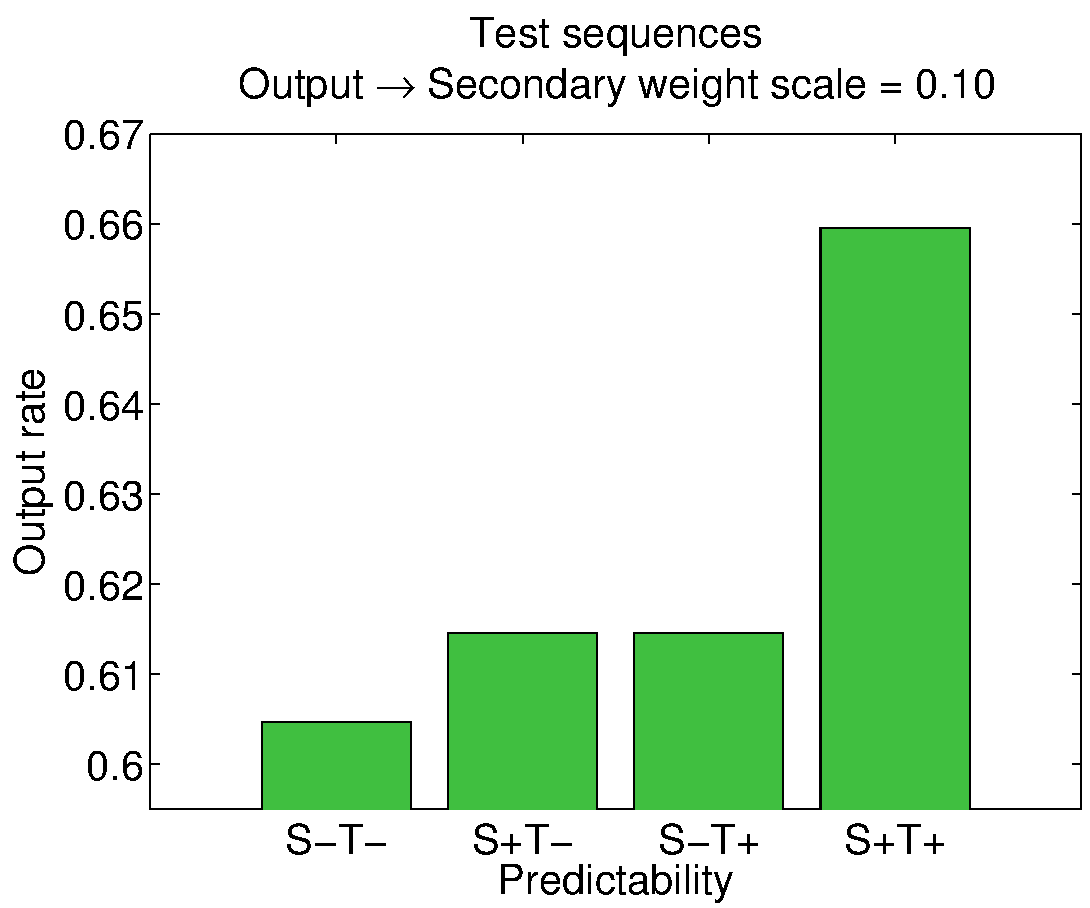
\includegraphics[width=80mm]{figs/chap_sims/sims_out_v2h_10_sterr.pdf}
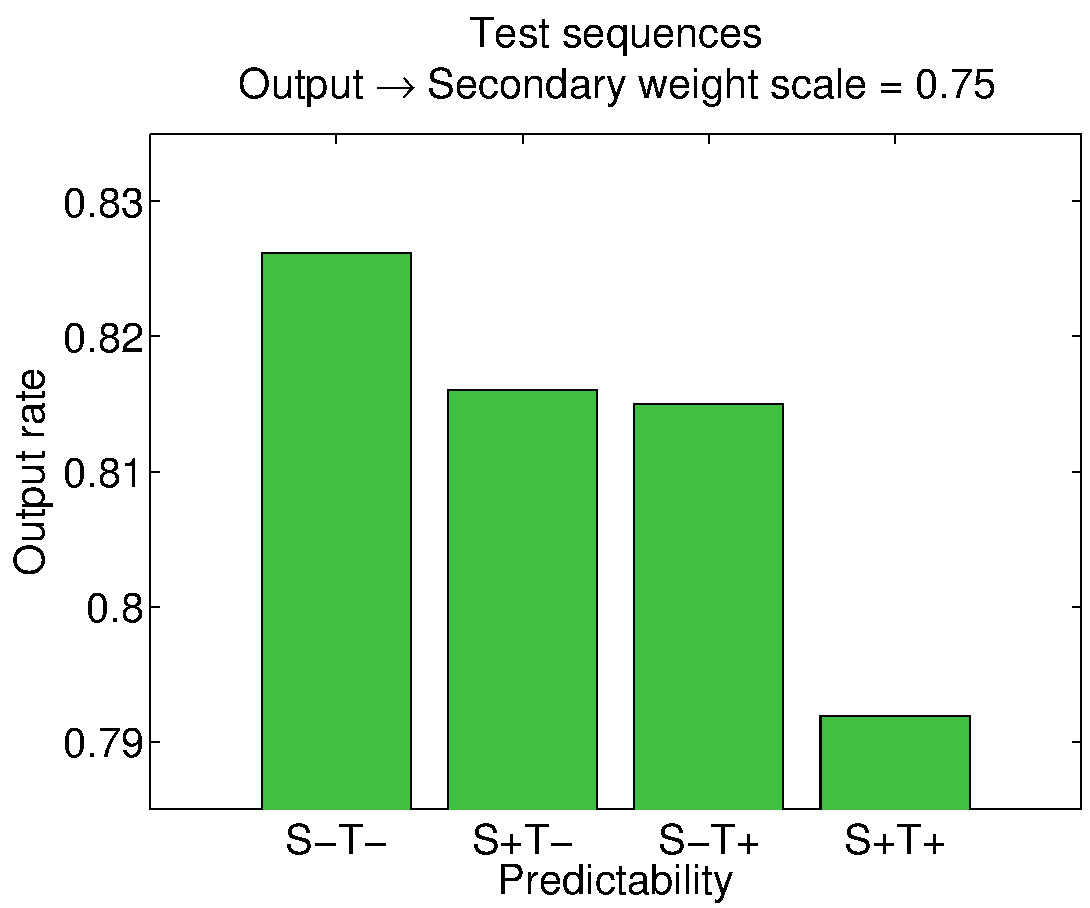
\includegraphics[width=80mm]{figs/chap_sims/sims_out_v2h_75_sterr.pdf}
\end{tabular}
\end{center}
\caption{Model results}{}
\label{fig:v1_v2_output_test}
\end{figure}

\section{Discussion}

\bibliographystyle{apa}
\bibliography{ccnlab}
\end{document}